\chapter{Angular: L'applicazione youCook}
\begin{figure}[H]
    \centering
 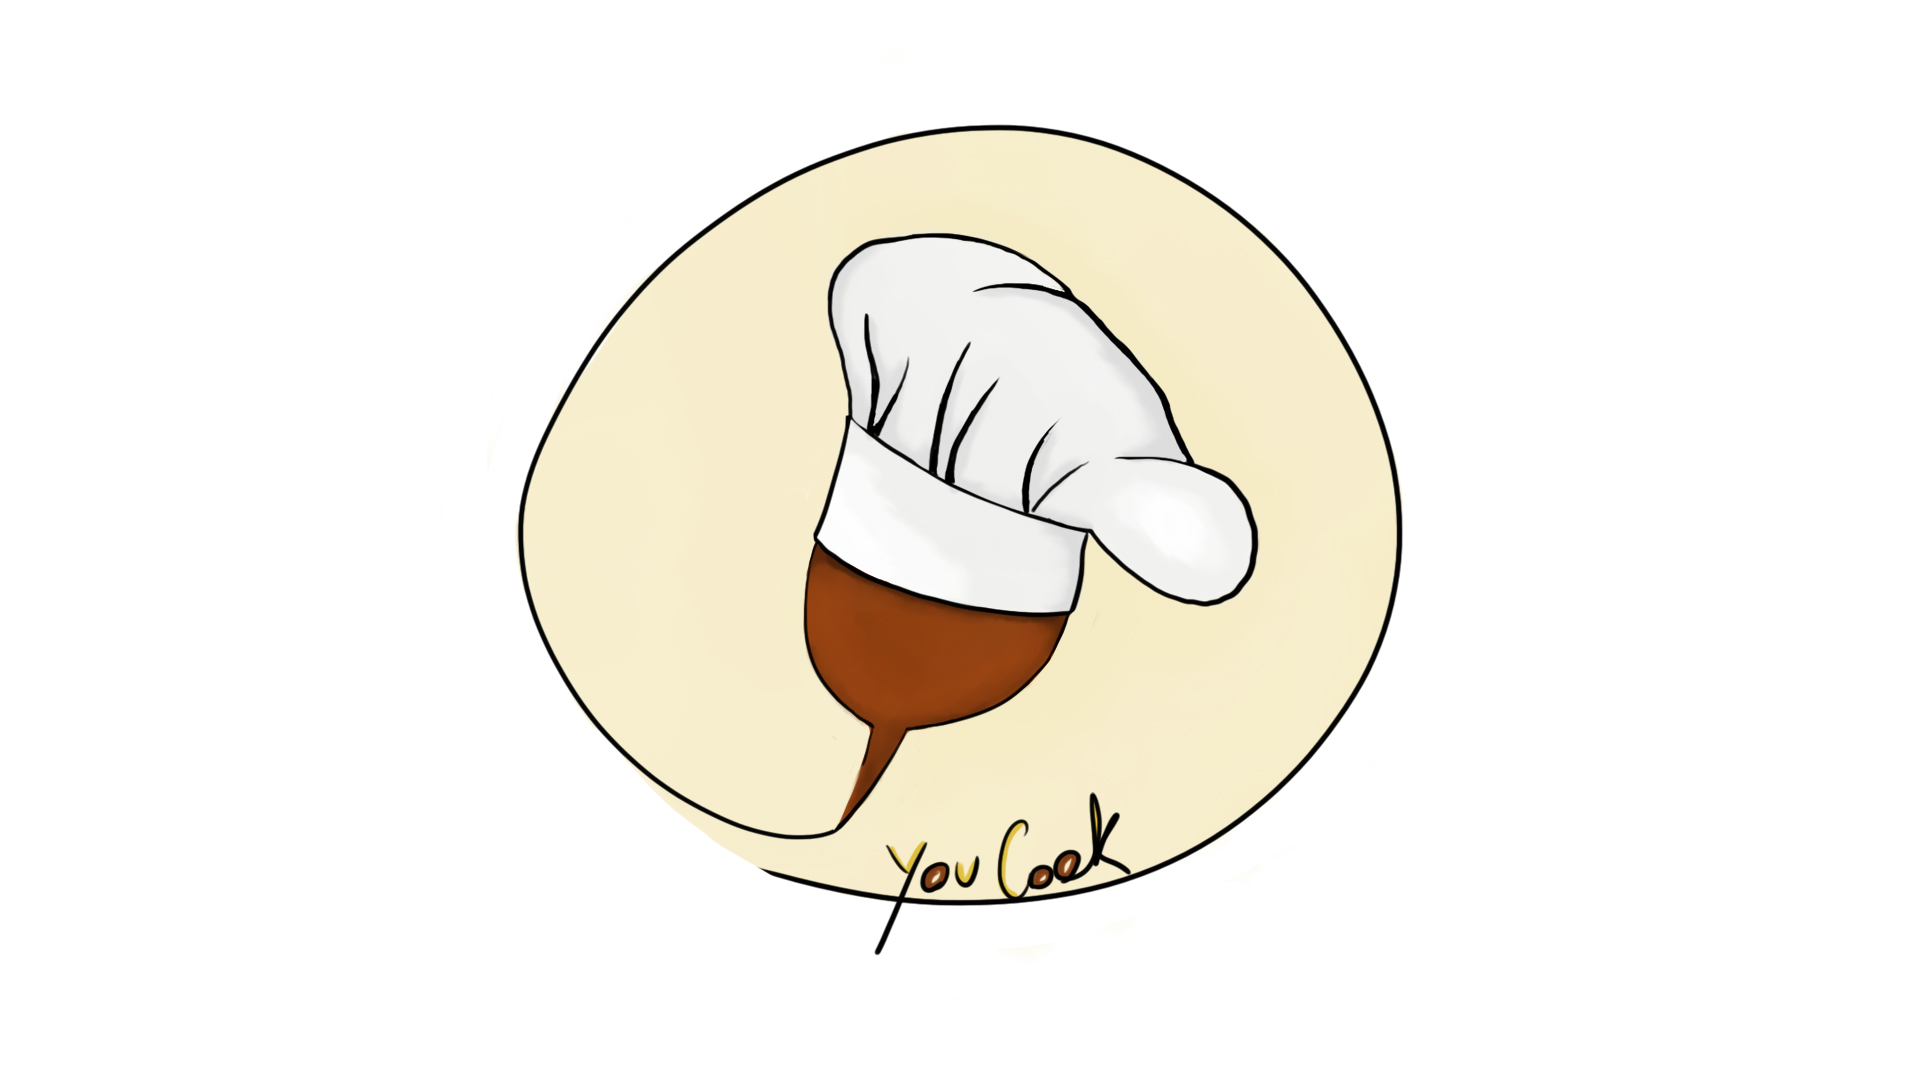
\includegraphics[scale=0.2]{resources/youCook_logo.jpg}
   \caption{logo dell'applicazione}
\end{figure}
\newpage
\section{YouCook: requisiti}
Al fine di mostrare le potenzialità della libreria segue il progetto di una applicazione per la gestione e condivisione delle ricette di cucina.
L' applicazione vuole soppiantare il classico "Libro mastro delle ricette" offrendo la possibilità di monitorare, aggiornare e gestire il proprio repertorio di ricette.
I requisiti della applicazione sono i seguenti:
\begin{itemize}
    \item L'utente deve poter gestire le proprie ricette, modificarle, creare e eliminarti
    \item L'utente deve poter effettuare ricerche in base agli ingredienti principali delle ricette
    \item L' utente deve poter creare gruppi famiglia all'interno dei quali selezionare fra le ricette il "Pasto del giorno" ovvero la ricetta che si intende realizzare per il pasto selezionato "pranzo, cena"
    \item all'interno del gruppo famiglia l'utente deve poter amministrare i membri

\end{itemize}
L'applicazione ha inoltre come obbiettivo quello di mettere in luce le potenzialità della strategia di change detection onPush.
\newpage
\subsection{Tabella dei requisiti}
\FloatBarrier
\begin{longtable}{|p{2.5cm}|p{9cm}|p{2.5cm}|}
\hline

\endfirsthead
\multicolumn{3}{c}%
{\tablename\ \thetable\ -- \textit{Continued from previous page}} \\
\hline
 \rowcolor{white}\textbf{ID} & \textbf{REQUISITO} & \textbf{TIPO} \\
\hline
\endhead
\hline \multicolumn{3}{r}{\textit{Continued on next page}} \\
\endfoot
\hline
\endlastfoot

\rowcolor{white}\textbf{ID} & \textbf{REQUISITO} & \textbf{TIPO} \\
         \hline
         R1F &L'applicazione deve fornire una funzionalità di registrazione agli utenti & Funzionale\\

         \hline
         R2F &L'applicazione deve dare la possibilità di aggiungere modificare e eliminare le proprie ricette&Funzionale \\

         \hline
         R3F &L'acquirente deve poter effettuare ricerche in base agli ingredienti & Funzionale \\

         \hline
         R4F &L'applicazione deve poter permettere all'utente di creare gruppi famiglia&Funzionale \\

         \hline
         R5F &L'applicazione deve poter permettere all'utente di amministrare i gruppi famiglia, rimuovendo o aggiungendo membri al gruppo &Funzionale \\

         \hline
         R6F & L'applicazione deve consentire all'utente di selezionare il "pasto del giorno"&Funzionale \\

\end{longtable}
\FloatBarrier
\newpage
\begin{figure}[H]
    \centering
 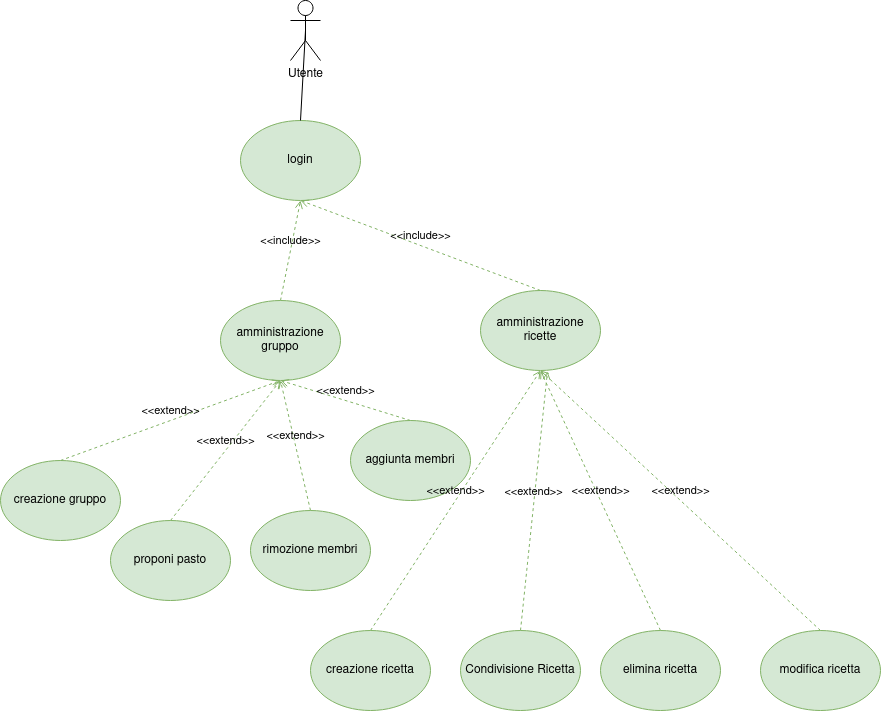
\includegraphics[scale=0.5]{resources/diagramma_casi_uso.drawio.png}
   \caption{Diagramma casi d'uso della applicazione}
\end{figure}
Il diagramma mette in luce le principali funzionalità fornite all'utente che, dopo la procedura di login, può visualizzare il proprio elenco di ricette e interagire con lo stesso  oppure visionare i membri del gruppo famiglia a lui associato.\section{YouCook: Scenari}

\FloatBarrier
\begin{longtable}{|p{4.5cm}|p{10cm}|}
\hline
\endfirsthead
\multicolumn{2}{c}%
{\tablename\ \thetable\ -- \textit{Continued from previous page}} \\
\hline
\endhead
\hline \multicolumn{2}{r}{\textit{Continued on next page}} \\
\endfoot
\hline
\endlastfoot


         \textbf{Titolo} & Login \\

         \hline
         \textbf{Descrizione} & Permette di accedere al sistema \\

         \hline
         \textbf{Attori} & Utente\\

         \hline
         \textbf{Relazioni} & Amministrazione gruppo, Amministrazione ricette \\
         \hline
         \textbf{Precondizioni} & L'utente deve essere già registrato\\

         \hline
         \textbf{Postcondizioni} & L'utente è autenticato nel sistema\\

         \hline
         \textbf{Scenario principale} &
            \begin{enumerate}
                \item All'utente viene presentata una maschera per l'inserimento delle credenziali
                \item L'utente inserisce i propri dati
                \item Il sistema verifica che i dati inseriti siano corretti
                \item Viene presentata la schermata principale all'utente
            \end{enumerate}
            \\


         \hline
         \textbf{Scenari alternativi} & Scenario a: Credenziali non riconosciute
            \begin{enumerate}
                \setcounter{enumi}{3}
                \item Il sistema non riconosce le credenziali inserite e presenta nuovamente la schermata iniziale di accesso
            \end{enumerate}
         \\

         \hline
         \textbf{Requisiti non funzionali} &\\

         \hline
         \textbf{Punti aperti} & \\



\end{longtable}
\FloatBarrier
\begin{longtable}{|p{4.5cm}|p{10cm}|}
\hline
\endfirsthead
\multicolumn{2}{c}%
{\tablename\ \thetable\ -- \textit{Continued from previous page}} \\
\hline
\endhead
\hline \multicolumn{2}{r}{\textit{Continued on next page}} \\
\endfoot
\hline
\endlastfoot


         \textbf{Titolo} & Amministrazione ricette \\

         \hline
         \textbf{Descrizione} & Permette di eliminare, modificare e aggiungere ricette  \\

         \hline
         \textbf{Attori} & Utente\\

         \hline
         \textbf{Relazioni} & creazione ricetta, modifica ricetta, elimina ricetta, login \\
         \hline
         \textbf{Precondizioni} & L'utente deve essere già autenticato\\

         \hline
         \textbf{Postcondizioni} &L'utente ha modificato il suo elenco di ricette\\

         \hline
         \textbf{Scenario principale} &
            \begin{enumerate}
                \item All'utente viene presentata una maschera con all'interno la lista delle ricette presenti nel suo inventario
                \item L'utente seleziona l'opzione che vuole effettuare (modifica, aggiunta o eliminazione)
                \item Il sistema porta a compimento l'azione descritta dall'utente
            \end{enumerate}
            \\


         \hline

         \hline
         \textbf{Requisiti non funzionali} &\\

         \hline
         \textbf{Punti aperti} & \\



\end{longtable}
\FloatBarrier
\begin{longtable}{|p{4.5cm}|p{10cm}|}
\hline
\endfirsthead
\multicolumn{2}{c}%
{\tablename\ \thetable\ -- \textit{Continued from previous page}} \\
\hline
\endhead
\hline \multicolumn{2}{r}{\textit{Continued on next page}} \\
\endfoot
\hline
\endlastfoot


         \textbf{Titolo} & Amministrazione Gruppo famiglia \\

         \hline
         \textbf{Descrizione} & Permette di eliminare e aggiungere membri al gruppo famiglia  \\

         \hline
         \textbf{Attori} & Utente\\

         \hline
         \textbf{Relazioni} & aggiunta membro, rimozione membro, login \\
         \hline
         \textbf{Precondizioni} & L'utente deve essere già autenticato\\

         \hline
         \textbf{Postcondizioni} &L'utente ha modificato il suo gruppo famiglia\\

         \hline
         \textbf{Scenario principale} &
            \begin{enumerate}
                \item All'utente viene presentata una maschera con all'interno la lista dei membri del suo gruppo famiglia
                \item L'utente seleziona l'opzione che vuole effettuare (aggiunta o eliminazione)
                \item Il sistema porta a compimento l'azione descritta dall'utente
            \end{enumerate}
            \\


         \hline

         \hline
         \textbf{Requisiti non funzionali} &\\

         \hline
         \textbf{Punti aperti} & \\



\end{longtable}\section{YouCook: modello del dominio}
\begin{figure}[H]
    \centering
 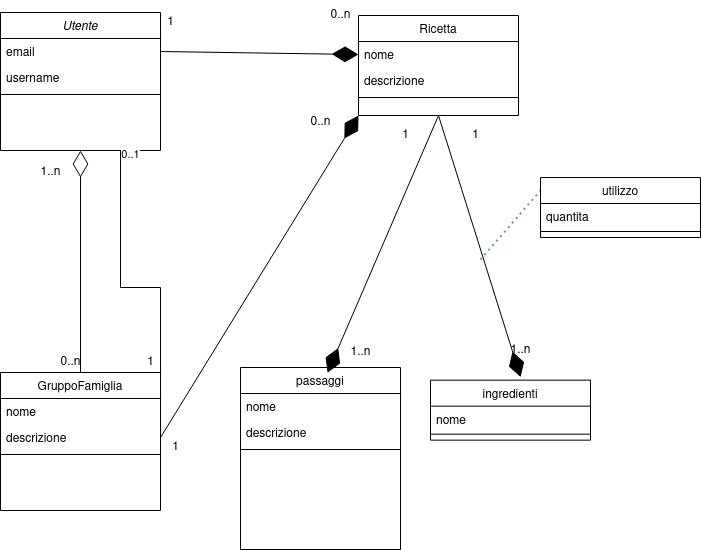
\includegraphics[scale=0.7]{resources/modello_del_dominio.drawio.png}
   \caption{Modello del dominio dell'applicazione}
\end{figure}
Il modello del dominio sopra rappresentato definisce le entità in gioco nell'applicazione. In particolare, vengono sfruttate due relazioni tra le classi utenti e gruppo famiglia per rappresentare i membri e il proprietario del gruppo. Viene inoltre utilizzata una classe d'associazione per rappresentare l'utilizzo del dato ingrediente in quella ricetta.\section{YouCook: progettazione}
La struttura dell'applicazione è la seguente
\begin{figure}[H]
    \centering
 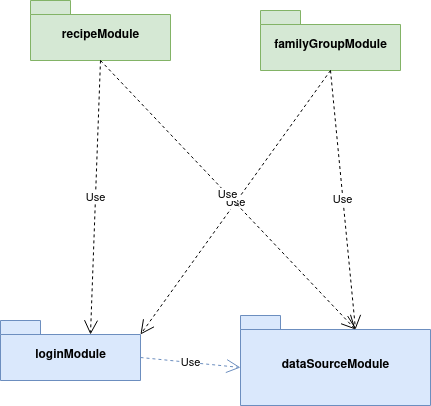
\includegraphics[scale=0.7]{resources/diagramma_package-diagramma_package.drawio.png}
   \caption{Diagramma dei package dell'applicazione}
\end{figure}
L'applicazione è composta da 4 module: i module recipe e familygroup implementano le rispettive funzionalità e sfruttano i servizi offerti dai module login e dataSource per autenticare gli utenti e realizzare la persistenza dei dati.
\begin{figure}[H]
    \centering
 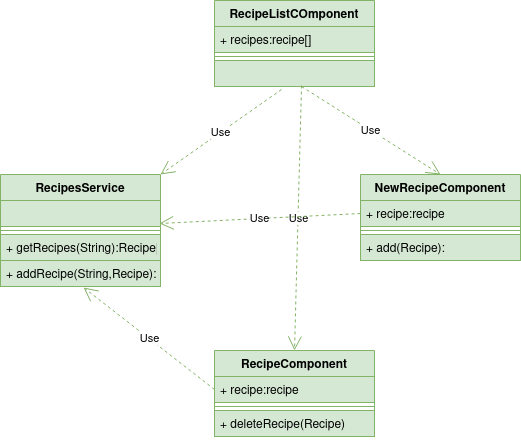
\includegraphics[scale=0.7]{resources/diagramma_package-recipe.drawio.png}
   \caption{Diagramma delle classi pakage recipe}
\end{figure}

\begin{figure}[H]
    \centering
 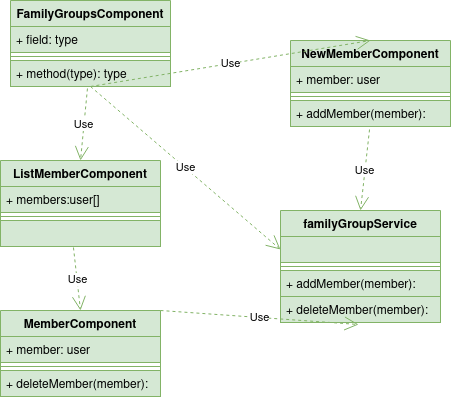
\includegraphics[scale=0.7]{resources/diagramma_package-FamilyGroup.drawio.png}
   \caption{Diagramma delle classi pakage FamilyGroup}
\end{figure}
I componenti dei package Recipe e FamilyGroup sfruttano la strategia di change detection onPush per aggiornare la lista di elementi mostrate nella view e sfruttano i rispettivi Service per interagire con la lista di elementi. Questi ultimi restituiscono a ogni modifica una nuova istanza della lista per attivare il meccanismo  di change detection.
\newline
È stato deciso di delegare la gestione della generazione degli oggetti a un service apposito, cosi da sollevare i componenti dalla necessità di implementare la logica applicativa. In questo modo i componenti possono concentrarsi sulla gestione della interfaccia e in caso si necessiti di modificare la logica con cui vengono gestiti i dati sarà sufficiente agire sul service.
\newpage
\begin{figure}[H]
    \centering
 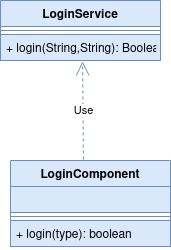
\includegraphics[scale=0.7]{resources/diagramma_package-login.drawio.png}
   \caption{Diagramma delle classi pakage login}
\end{figure}
\begin{figure}[H]
    \centering
 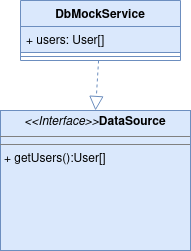
\includegraphics[scale=0.7]{resources/diagramma_package-dataSource.drawio.png}
   \caption{Diagramma delle classi pakage dataSource}
\end{figure}
Il package DataSource sfrutta il pattern strategy per implementare la persistenza verso i data store tramite l'interfaccia DataSource. In questo modo si astrae l'applicazione dalla gestione dello storage dei dati e consentire il recupero dei dati da datastore differenti.
\newline
I package login e datasource mettono ha disposizione una classe service per fornire le funzionalità agli altri componenti.




%- capitolo 1 e capitolo 2 vanno abbastanza bene, mentre il capitolo 3 è deboluccio.
%Riporti anche motivazioni più estese delle scelte fatte, screenshot dell'applicazione realizzata che la aiutino a descriverne le funzionalità. Servirebbero anche dati numerici sulle prestazioni di performance, ma forse a questo punto non ha più il tempo di farle...\section{YouCook: interfacce}
di seguito si riporta l'interfaccia principale della applicazione

\begin{figure}[H]
    \centering
 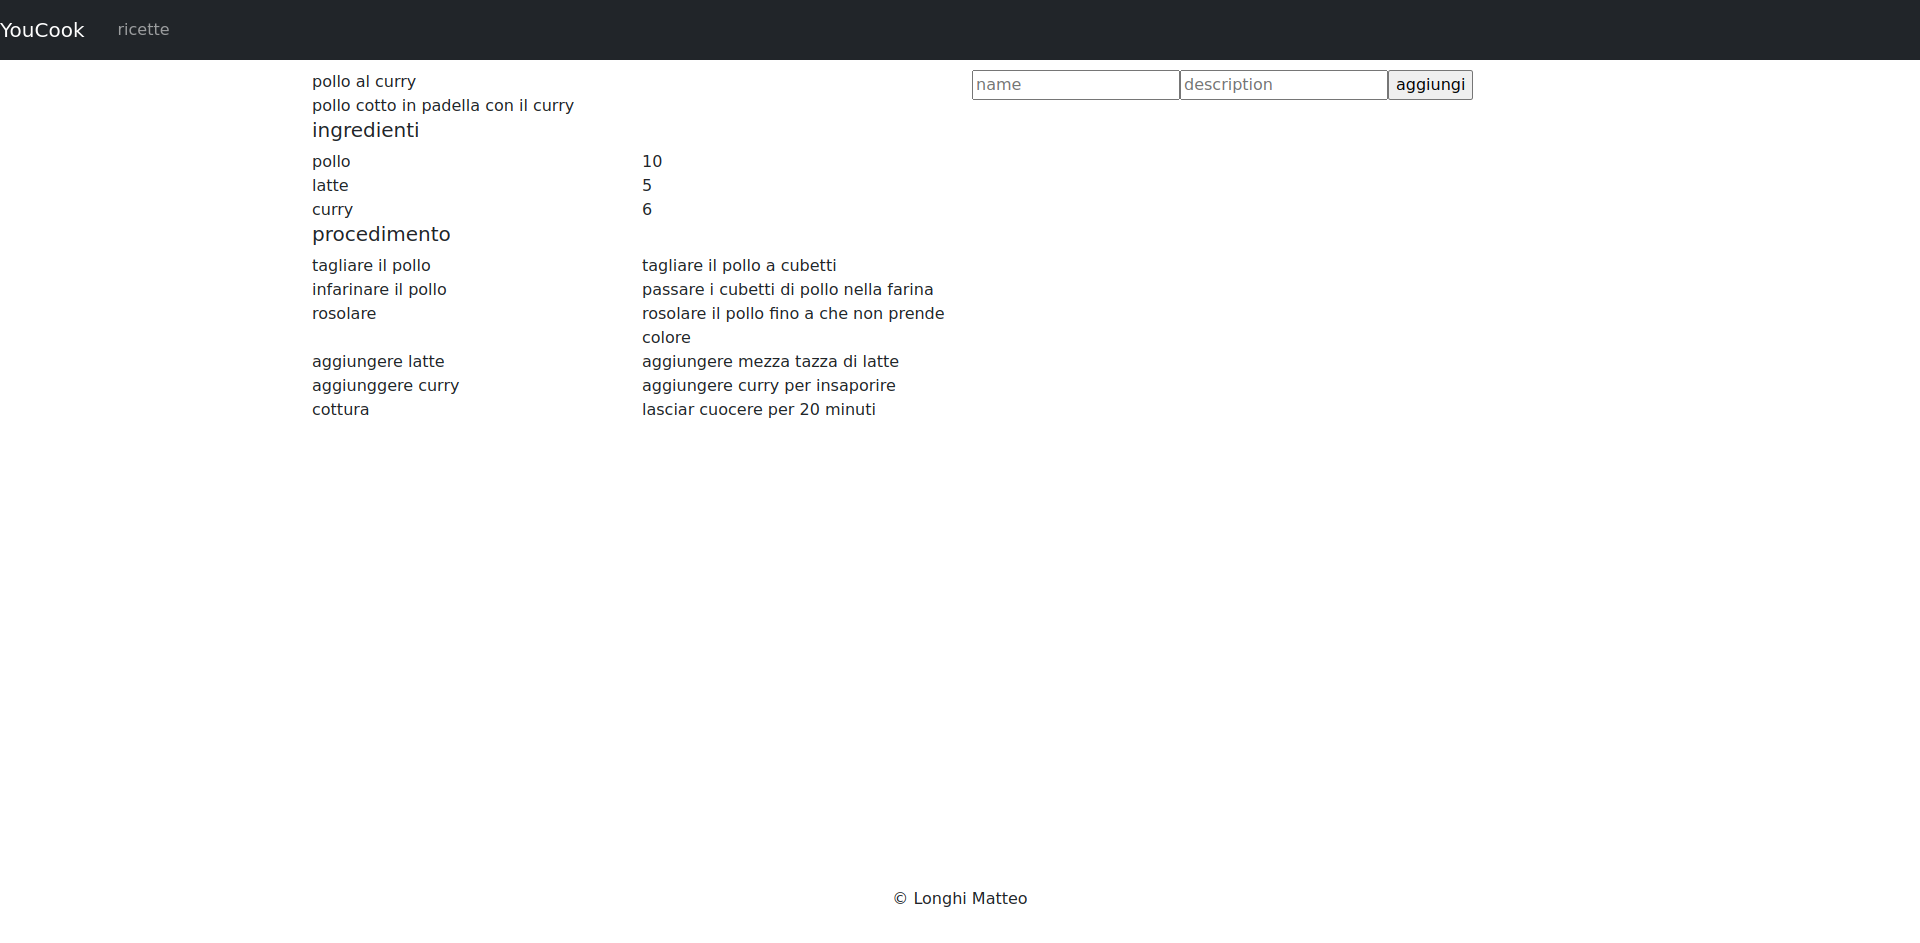
\includegraphics[scale=0.2]{resources/interfaccia-recipes.png}
   \caption{interfaccia sezione recipes dell'applicazione}
\end{figure}
L'interfaccia offre la possibilità di visionare l'elenco delle ricette e di aggiungerne di nuove tramite il form apposito.
L'elenco a destra viene renderizzato tramite la strategia onpush di change detection.
\newline
Il componente RecipesListComponent si registra a un osservabile messo a disposizione dal RecipesService che, alla modifica della lista di ricette da parte del NewRecipeComponent, emette una nuova lista di ricette attivando cosi il meccanismo di change detection
\newpage
codice NewRecipeComponent:
\begin{lstlisting}{typescript}
import { ChangeDetectionStrategy, Component, OnInit } from '@angular/core';
import { Recipe } from '../model/Recipe';
import { RecipesService } from '../recipes.service';

@Component({
  selector: 'app-recipes-list',
  changeDetection:ChangeDetectionStrategy.OnPush,
  templateUrl: './recipes-list.component.html',
  styleUrls: ['./recipes-list.component.css']
})
export class RecipesListComponent implements OnInit {
  public recipes?:Recipe[];
  constructor(private rs:RecipesService ){
  }
  ngOnInit(): void {
   this.recipes=this.rs.getRecipes();
   this.rs.recipesEvent.subscribe(recipes=>{
    this.recipes=recipes
   })
  }


}

\end{lstlisting}

\newpage
codice RecipeService;
\begin{lstlisting}{typescript}
import { EventEmitter, Injectable } from '@angular/core';
import { DatabaseService } from 'src/database.service';
import { Recipe } from './model/Recipe';
import { SessionService } from './session.service';

@Injectable({
  providedIn: 'root'
})
export class RecipesService {
private recipes?:Recipe[];
public recipesEvent:EventEmitter<Recipe[]>=new EventEmitter();
  constructor(private dbs:DatabaseService, private ss:SessionService ) {
    this.recipes=this.dbs.getUser(this.ss.getUsername())?.recipies;
  }
  public getRecipes(){
    return JSON.parse(JSON.stringify(this.recipes));

  }
  public addRecipes(r:Recipe ){
    this.recipes?.push(r);

    this.recipesEvent.emit(this.recipes);

  }
}
\end{lstlisting}
\section{YouCook: test prestazioni}
Sono stati anche eseguiti dei test sull'applicazione per verificarne i tempi di risposta
\begin{figure}[H]
    \centering
 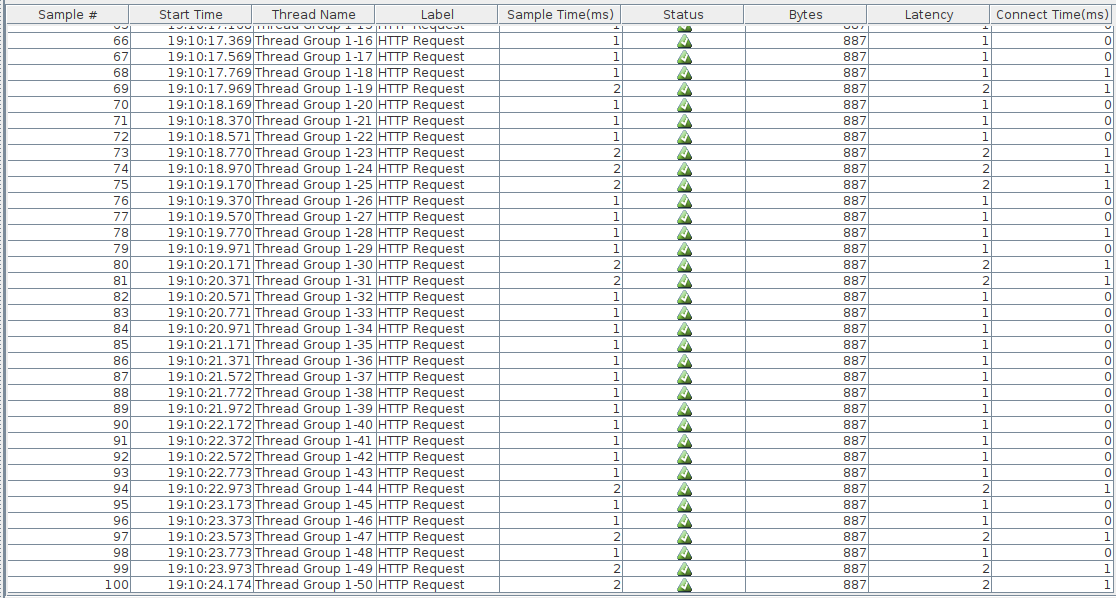
\includegraphics[scale=0.4]{resources/tests.png}
   \caption{Test effettuati per mezzo di jmeter}
\end{figure}
Il test eseguito prevedeva un pool di 50 thread, dal quale possiamo evincere che l'applicazione si comporta egregiamente sotto carico, totalizzando un tempo medio di risposta di circa 2 millisecondi (l'applicazione è stata testata in una rete locale)
